\section{楕円型境界の保持と相対 pants への交換}
\label{eb:section}

第\ref{acp:section}節と第\ref{kc:section}節の caps は、元の upper artificial cuts を埋めるが、
終点に genuine な elliptic boundary を作る。
その elliptic stratum は source の実際の境界ではなく、既に full normal disk を持つ。
従って、その full germ を固定したまま別の領域を追加する方法では、基底の片側性を消せない。
本節ではこの点を確認した後、cap の内部の fibration を変更し、
元の outer whole collar を厳密に保持する相対 pants を明示する。
この交換は一つの elliptic face を一つの hyperbolic family と二つの regular ports に変える。
新しい ports の先の充填を完了する主張ではない。

\subsection{Full elliptic germ を保持する接続の限界}

\begin{proposition}[Compact elliptic germ の片側性]\label{eb:persistence}
$M$ を Hausdorff な六次元多様体、$\pi:M\to B$ を connected fibers を持つ quotient map とし、
$B$ は Hausdorff とする。
ある開集合 $U\subset M$ に
\[
 U\simeq P\times T^2\times D^2,\qquad P\subset\RR^2
\]
という full neighborhood があり、$U$ 上の $\pi$ の fiber relation が
\[
 f(I_1,I_2,\alpha_1,\alpha_2,z)
   =(I_1,I_2,\pi|z|^2)
\]
の fiber relation と一致すると仮定する。
このとき $U$ は $\pi$-saturated であり、その quotient は $B$ の開集合として
$P\times[0,\varepsilon)$ と同相である。
特に、この full germ を固定した外部領域の追加では、$z=0$ に対応する elliptic face を消せない。
\end{proposition}

\begin{proof}
$f$ の各 fiber $L$ は $T^3$ または $T^2$ であり compact である。
仮定より $\pi^{-1}(\pi(L))\cap U=L$ だから、$L$ は global fiber の中で開いている。
また $M$ が Hausdorff で $L$ が compact なので、同じ fiber の中で閉じている。
Global fiber の connectedness により $\pi^{-1}(\pi(L))=L$ となる。
全ての $L$ に適用すると $U$ は saturated である。
Quotient map の saturated open set の像は開集合なので、$\pi(U)$ は開いている。
制限 $\pi|_U$ と $f$ は同じ equivalence relation を持つ quotient maps だから、
$\pi(U)$ は $P\times[0,\varepsilon)$ と同相である。
\end{proof}

Compact source から Hausdorff base への continuous surjection、あるいは proper な連続全射では、
quotient-map 条件は自動である。
命題は一つの点での quadratic normal form だけを仮定するものではなく、
compact orbit と whole nearby tori の full germ を仮定する。
今回の caps はこの explicit product を持つ。
一般の nondegenerate compact singular orbit に対する normal form は
Miranda--Zung \cite[Theorem 2.1]{miranda-local} を参照されたい。

同じ scalar value を遠方の別の $T^2$ に割り当てても、connected-component quotient は両者を同一視しない。
Base だけを貼り合わせてこれを強制すれば、seam の fiber は不連結となる。
また source の二つの elliptic strata 自体を同一視すれば、横断方向は $D^2\vee D^2$ となり、
source は $\RR^4\times(D^2\vee D^2)$ 型で smooth 六次元多様体ではない。
この局所空間の相対 homology は次数 $6$ で $\ZZ^2$、次数 $5$ で $\ZZ$ となる。

Base にも位相的な区別がある。
$k$ 本の半直線を一つの頂点で結んだ空間を $Y_k$ とすると、頂点に対応する $b$ で
\[
 H_3\bigl(\RR^2\times Y_k,
       (\RR^2\times Y_k)\setminus\{b\};\ZZ\bigr)
   \simeq\ZZ^{k-1}.
\]
これは $Y_k$ の頂点を除いた空間が $k$ 個の contractible components を持つことから従う。
従って elliptic face、regular interior、true $Y$ branch は順に rank $0,1,2$ で区別され、
単なる labels の変更では互いに移らない。
Parameter 側面の接続だけでも、elliptic face の相対内部は変わらない。

\subsection{Cap の product coordinates と内側の変更}

以下の角度は全て周期 $1$ とする。
Compact contractible parameter region $P$ と、その近傍上の smooth function $g>0$ に対し、
\begin{equation}\label{eb:product-cap}
 \begin{split}
 \mathcal C_g
   &=\{I=(I_1,I_2)\in P,\ \alpha\in T^2,\ 0\le p\le g(I)\},\\
 \lambda_0&=I_1d\alpha_1+I_2d\alpha_2+p\,d\theta,
 \qquad z=\sqrt{p/\pi}\,e^{2\pi i\theta},\qquad \omega=d\lambda_0
 \end{split}
\end{equation}
という product cap を考える。
$p\,d\theta$ は $z=0$ でも滑らかである。
その元の fibration は $(I_1,I_2,p)$ の levels、またはこれらの smooth な labels で表す。

$\delta$ cap では、整形後の coordinates で
\[
 I_1=b+sA_x,\qquad I_2=sA_z,\qquad p=sM,\qquad \theta=\theta_y
\]
と取れる。
Natural cap の flat model では
\[
 I_1=K_H,\qquad I_2=K_J,\qquad p=\rho_w,\qquad \theta=\chi
\]
である。
$SU(2)$ suspension と upper straightening の後は、これらの transported coordinates を使う。
Primitive に現れる exact term は、以下の action と cycle relation を変えない。

\begin{theorem}[Outer whole collar を固定する actual pants]\label{eb:pants}
式\eqref{eb:product-cap}の cap に対し、二つの小さい regular disk sublevels を除いた部分領域
$\mathcal C_g^{\rm pants}\subset\mathcal C_g$ と、その上の Lagrangian fibration がある。
この fibration は次の性質を持つ。
\begin{enumerate}
\item 元の outer whole collar と、その collar 上の全ての scalar labels を厳密に保持する。
二つの shared actions $I_1,I_2$ も保持する。
\item Regular fibers は $T^3$、各 parameter $I$ 上の唯一の singular fiber は
$T^2\times(S^1\vee S^1)$ であり、その singular orbit は nondegenerate rank-two hyperbolic 型である。
Connected-fiber quotient は true $Y$ branch を持ち、elliptic fibers を持たない。
\item 二つの新しい regular $T^3$ ports を持つ。Parameter 側面は自由なまま残る。
この block の connected-fiber quotient は Hausdorff である。
\end{enumerate}
構成は一つの full product cap の内部で行うため、actual cap の symplectic embedding をそのまま使える。
\end{theorem}

\begin{proof}
$0<R<\min_P g$ を固定する。
$\chi:[0,\infty)\to[0,1]$ を、$p\le R/3$ で $1$、$p\ge2R/3$ で $0$ となる smooth cutoff とし、
\[
 C_\chi=1+R\sup|\chi'|,\qquad
 0<\nu<\frac{R}{10C_\chi}
\]
と選ぶ。$w=\sqrt p\,e^{2\pi i\theta}=\sqrt\pi z$ と書き、
\begin{equation}\label{eb:morse-function}
 h_\nu(w)=p^2-2\nu\chi(p)\operatorname{Re}(w^2)+\nu^2
         =p^2-2\nu p\chi(p)\cos(4\pi\theta)+\nu^2
\end{equation}
と定める。
これは Cartesian coordinates で滑らかであり、$p\le R/3$ で $|w^2-\nu|^2$、
$p\ge2R/3$ で $p^2+\nu^2$ となる。
$p\ge R/3$ では
\begin{equation}\label{eb:radial-positive}
 \partial_p h_\nu
 =2p-2\nu\bigl(\chi+p\chi'\bigr)\cos(4\pi\theta)
 \ge\frac{2R}{3}-2\nu C_\chi>0.
\end{equation}
ここで $\chi'$ の support は $p<R$ に含まれる。
従ってこの領域には critical points がない。

$p<R/3$ では、critical points は $w=\pm\sqrt\nu$ と $w=0$ の三つだけである。
最初の二点は値 $0$ の minima であり、quadratic term は $4\nu|dw|^2$ となる。
$w=0$ では値が $\nu^2$、Hessian は $(\operatorname{Re}w,\operatorname{Im}w)$ で
$\operatorname{diag}(-4\nu,4\nu)$ となり、nondegenerate saddle である。

次に smooth strictly increasing な $\varphi:[0,\infty)\to[0,\infty)$ を、
\[
 \varphi(0)=0,\qquad
 \varphi(t)=\sqrt{t-\nu^2}\quad
 \left(t\ge (2R/3)^2+\nu^2\right)
\]
となるよう選ぶ。
実際、右辺の正の derivative を threshold の短い collar から左へ正に延長し、
残る区間の積分が $2R/3$ となるよう正の bump で調整してから積分すればよい。
最初の collar を短くすれば、その強制される積分を $2R/3$ より小さくできる。
すると
\[
 H=\varphi\circ h_\nu
\]
は $p\ge2R/3$ で厳密に $p$ と一致し、同じ三つの critical points を持つ。
$p\le R/3$ では $h_\nu\le(R/3+\nu)^2<(2R/3)^2+\nu^2$ であり、
$R/3\le p\le2R/3$ では式\eqref{eb:radial-positive}を使えるので、
$p\le2R/3$ の全体で $0\le H\le2R/3$ である。

元の third label が $q_{\rm old}(I,p)$ で表される場合は
\begin{equation}\label{eb:old-label}
 q_{\rm new}(I,w)=q_{\rm old}\bigl(I,H(w)\bigr)
\end{equation}
と置く。
元の $q_{\rm old}$ が $p$ に関して strictly monotone なら、同じ level partition を得る。
Parameter に依存するこの再表示は $p\ge2R/3$ で元の label と厳密に一致する。
他の scalar labels も $(I,p)$ の関数として同様に合成できる。
従って foliation だけでなく、元の outer collar 上の functions 自体を保持できる。

$0<\eta<\nu^2$ を固定し、例えば $\eta=\nu^2/4$ とする。
$\{h_\nu\le\eta\}$ は二つの互いに素な closed disks $D_+,D_-$ からなり、
\[
 p\le\nu+\sqrt\eta<2\nu<R/3
\]
に入るので、cutoff による変更を受けない。
そこで
\begin{equation}\label{eb:pants-domain}
 \mathcal C_g^{\rm pants}
 =\mathcal C_g\setminus
  \bigl(P\times T^2\times\operatorname{int}(D_+\cup D_-)\bigr)
\end{equation}
とする。
これは $P$ 上で $T^2\times\text{pair of pants}$ 型であり、$(I_1,I_2,H)$ は可換である。
Normal direction の level circles と shared $T^2$ の積は Lagrangian $T^3$ となる。

Critical level は
\begin{equation}\label{eb:lemniscate}
 p=2\nu\cos(4\pi\theta)\ge0
\end{equation}
で表される figure-eight であり、全て $p\le2\nu<R/3$ に入る。
二つの lobes を交換する quotient は取らず、同じ free $T^2$ との積を用いる。
従って singular fiber は whole $T^2\times(S^1\vee S^1)$ で、Reeb vertex は三価である。
$\eta<h_\nu<\nu^2$ では二つ、$h_\nu>\nu^2$ では一つの circle component がある。
外側の positive radial derivative により、他の critical points や components は生じない。
Compact Morse surface の connected-level quotient は有限 graph であり、
ここでは二つの低い枝と一つの高い枝を持つ $Y$ となる。
Parameter family は同じ fixed core model を使い、outer radial segment の長さだけが $g(I)$ に依存する。
従ってその quotient は $P$ 上の Hausdorff な collared family である。
二つの新しい boundary components は $h_\nu=\eta$ の regular ports であり、
元の outer collar は全て固定されている。
\end{proof}

\begin{corollary}[24か所の同時交換]\label{eb:all24}
系\ref{acp:assembly-caps}の全24 $\delta$ caps、または系\ref{kc:mixed-caps}の混合24 caps に対し、
定理\ref{eb:pants}を同時に適用できる。
元の curve block と全 annular blocks、その whole fibers、marked periods、focus、true saddle を変更せず、
upper caps の24 elliptic faces を、24個の追加 hyperbolic families と48本の新 regular $T^3$ ports に交換する。
新しい領域は元 cap の部分領域なので、既存 assembly との非交差は保持される。
\end{corollary}

\begin{proof}
各 cap の full product coordinates を用い、個別に $R,\nu,\eta$ を選ぶ。
全変更は cap の内部にあり、attachment collar は固定される。
Actual symplectomorphisms で pull back すれば各新 block は元 cap の部分集合となるため、
前節までの finite assembly の非交差がそのまま適用される。
元の quotient への接続も同じ regular collars を使う。
\end{proof}

この系では、各 cap から二つの disk families を除いたため、fibration の定義域は小さくなる。
除いた領域は actual $X_\tau$ の中に存在するが、現在の fibration domain には含めていない。
それらを元の radial minima で戻せば elliptic faces が再び現れる。
また、この系は merged caps の elliptic faces、parameter 側面、他の geometric corners を処理していない。
48本の新 ports を全体構成へ接続することと、whole $X_\tau$ の Hausdorff quotient は未証明である。

\begin{figure}[htbp]
\centering
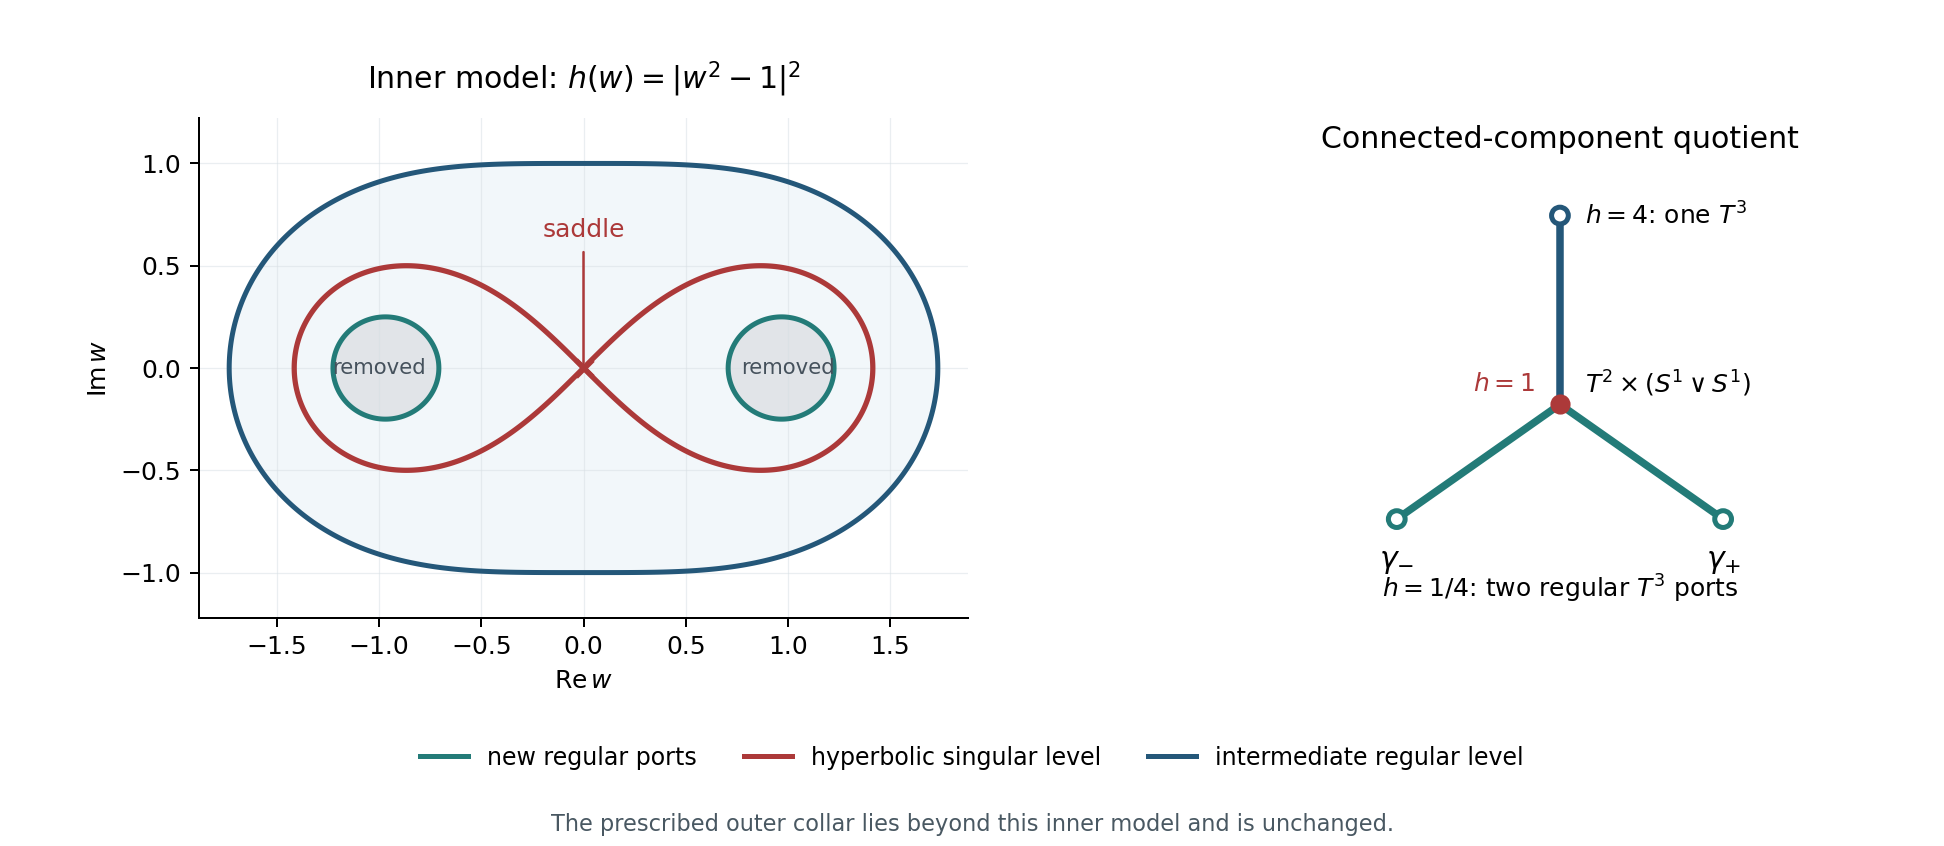
\includegraphics[width=\textwidth]{elliptic_pants_model.png}
\caption{Cutoff が恒等な内側での $|w^2-\nu|^2$ と connected-component quotient。
図は $\nu=1$、内側 cut $\eta=1/4$ の規格化であり、青線 $h=4$ は中間の正則 level である。
元の prescribed outer collar は図の範囲外にあり、相対構成では厳密に保持する。
灰色の二つの disk interiors を定義域から除く。表示していない shared $T^2$ との積を取ると、
赤い特異 level は $T^2\times(S^1\vee S^1)$ となる。}
\label{eb:inner-figure}
\end{figure}

\subsection{新しい ports の作用と cycle relation}

Outer circle を $\gamma_o$、二つの inner circles を $\gamma_+,\gamma_-$ とし、
いずれも normal disk の面積形式に関して反時計回りに向ける。
Inner circles のこの向きは、pants の boundary orientation と逆である。
Shared angles $\alpha_1,\alpha_2$ を固定して取れば
\begin{equation}\label{eb:cycle-relation}
 [\gamma_o]=[\gamma_+]+[\gamma_-]
 \quad\text{in }H_1(\text{pair of pants};\ZZ)
\end{equation}
となり、shared $T^2$ の cycle は付加されない。
$\gamma_\pm$ はそれぞれ primitive であり、元の filled cap では取り除いた actual symplectic disks を張る。

\begin{proposition}[Lobe actions の明示式]\label{eb:lobe-action}
$0<t<\nu^2$ における二つの sublevel disks は同じ面積
\begin{equation}\label{eb:lobe-integral}
 \mathcal A_\nu(t)
   =\frac1{4\pi}\int_{|u-\nu|\le\sqrt t}\frac{dA_u}{|u|}
\end{equation}
を持ち、
\begin{equation}\label{eb:lobe-bounds}
 \frac{t}{4(\nu+\sqrt t)}
 \le\mathcal A_\nu(t)
 \le\frac{t}{4(\nu-\sqrt t)}
\end{equation}
となる。
Saddle における各 lobe の面積と、上側 circle の action limit は
\begin{equation}\label{eb:saddle-actions}
 \mathcal A_\nu(\nu^2)=\frac\nu\pi,
 \qquad \mathcal A_o(\nu^2)=\frac{2\nu}{\pi}
     =\mathcal A_+(\nu^2)+\mathcal A_-(\nu^2).
\end{equation}
Outer port $p=g(I)$ と二つの inner ports $h_\nu=\eta$ では
\begin{equation}\label{eb:port-actions}
 \int_{\gamma_o}\lambda_0=g(I),\qquad
 \int_{\gamma_\pm}\lambda_0=\mathcal A_\nu(\eta)>0,
 \qquad
 \operatorname{Area}(\text{pants}_I)=g(I)-2\mathcal A_\nu(\eta).
\end{equation}
\end{proposition}

\begin{proof}
$w$-plane の Euclidean area を $dA_w$ とすると、normal symplectic form は
$dp\wedge d\theta=dA_w/\pi$ である。
$u=w^2$ は各 sublevel disk から $|u-\nu|\le\sqrt t$ への diffeomorphism で、
Jacobian は $4|u|$ だから式\eqref{eb:lobe-integral}を得る。
積分領域で $\nu-\sqrt t\le|u|\le\nu+\sqrt t$ を使うと式\eqref{eb:lobe-bounds}となる。
Critical lobe には式\eqref{eb:lemniscate}を直接用い、
\[
 \int_{-1/8}^{1/8}2\nu\cos(4\pi\theta)\,d\theta=\frac\nu\pi
\]
を得る。もう一方の lobe も同じであり、upper sublevel の面積はその和に連続して収束する。
各 regular circle での primitive period は、それが囲む normal disk の面積である。
Outer circle では $p=g(I)$ が一定なので period は $g(I)$。
Inner circles では式\eqref{eb:lobe-integral}となり、最後の式は Stokes の定理である。
\end{proof}

$\eta=\nu^2/4$ と取れば $\nu/24\le\mathcal A_\nu(\eta)\le\nu/8$ である。
Saddle における三つの action limits は厳密に加法的だが、
異なる高さにある三つの boundary actions の差には、式\eqref{eb:port-actions}の pants 面積が入る。
また $\mathcal A_\nu'(t)>0$ であり、saddle に近づく derivative の発散は通常の hyperbolic behavior である。
これは $h_\nu$ 自体の滑らかさの問題ではない。

\subsection{Primitive discrepancy の二つの ports への分配}

\begin{proposition}[Primitive の相対延長条件]\label{eb:primitive-split}
Outer collar に指定した primitive が
\begin{equation}\label{eb:outer-primitive}
 \lambda_{\rm old}
 =\lambda_0+c_1^T d\alpha_1+c_2^T d\alpha_2+c_o d\theta+dF
\end{equation}
と書けるとする。$c_1^T,c_2^T,c_o$ は connected parameter domain 上の定数である。
任意の定数 $c_+,c_-$ に対し、同じ $\omega$ の smooth primitive を pants 全体に延長し、
outer collar では $\lambda_{\rm old}$ と厳密に一致させ、inner meridian periods を
\begin{equation}\label{eb:inner-periods}
 \mathcal A_\nu(\eta)+c_+,\qquad \mathcal A_\nu(\eta)+c_-
\end{equation}
とするための必要十分条件は
\begin{equation}\label{eb:period-split}
 c_++c_-=c_o
\end{equation}
である。Shared periods は $I_j+c_j^T$ となる。
\end{proposition}

\begin{proof}
二つの中心 $\pm\sqrt\nu$ は除いた disks の内部にあるので、
\[
 \zeta_0=c_+\frac{d\arg(w-\sqrt\nu)}{2\pi}
            +c_-\frac{d\arg(w+\sqrt\nu)}{2\pi}
\]
は pants 全体で滑らかな closed one-form である。
その inner periods は $c_+,c_-$、outer period は $c_++c_-=c_o$ となる。
Outer annulus で $\zeta_0-c_o d\theta$ は period が零だから exact である。
これを $df$ と書き、その annulus に support を持ち outer collar で $1$ となる cutoff $\kappa$ により
\[
 \zeta=\zeta_0-d(\kappa f)
\]
とすれば、$\zeta=c_o d\theta$ が outer collar で厳密に成り立つ。
同じく $F$ を outer collar から cutoff を使って延長し、
\[
 \lambda_{\rm ext}
 =\lambda_0+c_1^T d\alpha_1+c_2^T d\alpha_2+\zeta+d\widetilde F
\]
と定めれば所要の primitive を得る。
逆に任意の延長の $\lambda_0$ との差は closed であり、
式\eqref{eb:cycle-relation}により式\eqref{eb:period-split}が必要となる。
また shared cycles は全 domain で同じ homology classes なので、shared periods も記載した通りである。
\end{proof}

式\eqref{eb:outer-primitive}は、outer collar の三つの marked periods が一致すれば、
残る closed difference が exact となることを明示している。
ここで $P$ が contractible なので、collar の $H^1$ は三つの torus cycles で尽くされる。
閉形式の periods は parameter に沿って局所一定であり、$c_\pm$ を自由な parameter-dependent functions に
置き換えてよいわけではない。

$\delta$ cap では元の primitive が filled disk 全体へ既に延びているので、
そのまま制限して $c_o=c_+=c_-=0$ とできる。
この場合、二つの inner periods は共に正の $\mathcal A_\nu(\eta)$ となる。

\begin{corollary}[Natural cap の discrepancy]\label{eb:natural-periods}
第\ref{kc:section}節の natural cap で $r=A-I_i^0$ と置く。
Transported flat angles を使えば、outer collar で $\theta_x=\alpha_1+\theta$ となり、
exact term を除いて
\[
 \lambda_{\rm old}=\lambda_{\rm cap}-r(d\alpha_1+d\theta)
\]
である。
従って元の primitive は pants 全体へ延長でき、二つの inner corrections は
\[
 c_++c_-=-r
\]
を満たす任意の定数に選べる。
Shared periods は $I_1-r,I_2$ であり、二つの inner meridian periods を同時に正にできる必要十分条件は
\begin{equation}\label{eb:both-positive}
 2\mathcal A_\nu(\eta)>r
\end{equation}
である。
\end{corollary}

\begin{proof}
Flat cap で $\alpha_1=\theta_u+\theta_v$、$\theta=\theta_w-\theta_u-\theta_v$ なので
$\theta_x=\theta_w=\alpha_1+\theta$ となる。
第\ref{kc:section}節の primitive difference は $r\,d\theta_x$ であり、
$SU(2)$ suspension と最後の inverse straightening を通して同じ boundary periods が保持される。
従って命題\ref{eb:primitive-split}で $c_1^T=-r,c_2^T=0,c_o=-r$ とすればよい。
二つの inner periods の和は $2\mathcal A_\nu(\eta)-r$ なので、両方が正なら式\eqref{eb:both-positive}が必要である。
逆にこの式が成り立てば $c_+=c_-=-r/2$ と取れば両方が正になる。
\end{proof}

式\eqref{eb:both-positive}が失敗しても regular $T^3$ port 自体への障害ではない。
Regular port の marked primitive period は負でもよい。
障害となるのは、その同じ oriented meridians を正面積の symplectic disks で埋め、
指定 primitive を disks 全体へ滑らかに延ばす条件を追加した場合である。
Pants への交換は discrepancy を二つの穴へ運ぶが、その総和を消さない。

\subsection{Hyperbolic fiber まで延びる周期的作用の格子}

新しい pants は shared $T^2$ を保つが、outer torus の第三の周期的作用まで保存するわけではない。
この差は、saddle に近づく normal period の発散で厳密に検出できる。

\begin{proposition}[延長可能な周期作用は shared lattice]\label{eb:periodic-lattice}
定理\ref{eb:pants}の product model で、外側 regular tori 上の cycle を
\[
 v=m_1e_1+m_2e_2+n\gamma_o\qquad(m_1,m_2,n\in\ZZ)
\]
とする。ここで $e_j$ は $\alpha_j$ の周期 $1$ orbit、$\gamma_o$ は positive normal circle である。
この cycle を生成する fibrewise Hamiltonian $S^1$ action の generator が、
whole hyperbolic singular fiber まで連続に延びる必要十分条件は $n=0$ である。
従って滑らかに延びる周期作用の格子は $\ZZ e_1\oplus\ZZ e_2$ である。
同じ結論は fibrewise symplectic $S^1$ actions にも成り立つ。
\end{proposition}

\begin{proof}
$t>\nu^2$ が十分近ければ、whole sublevel disk $\{h_\nu\le t\}$ は cutoff が $1$ の領域に入る。
$u=w^2$ は $|u-\nu|\le\sqrt t$ 上で、branch point を除き二重被覆である。
従って outer action とその derivative は
\begin{align}
 \mathcal A_o(t)
   &=\frac1{2\pi}\int_{|u-\nu|\le\sqrt t}\frac{dA_u}{|u|},
       \label{eb:outer-action-integral}\\
 T_o(t)=\mathcal A_o'(t)
   &=\frac1{4\pi}\int_0^{2\pi}
       \frac{d\phi}{|\nu+\sqrt t\,e^{i\phi}|}.
       \label{eb:outer-period}
\end{align}
面積の derivative $T_o(t)$ は、$h_\nu$ の Hamiltonian flow が normal circle を一周する時間である。
$\phi=\pi$ の近くで分母は
\[
 \sqrt{(\sqrt t-\nu)^2+2\nu\sqrt t\,(1+\cos\phi)}
\]
となる。従って $t\downarrow\nu^2$ で積分は logarithmically に発散し、$T_o(t)\to+\infty$ である。

Regular chamber 上では $(I_1,I_2,\mathcal A_o(h_\nu))$ が action coordinates になる。
Fibrewise symplectic vector field の $\iota_X\omega$ は closed であり、
Lagrangian fiber 上で零なので、局所的には base 上の closed one-form の pullback である。
従ってその係数は torus angles に依存しない。
周期 $1$ の flow の cycle が $v$ であることから、その Hamiltonian は局所定数を除いて
\[
 m_1I_1+m_2I_2+n\mathcal A_o(h_\nu)
\]
であり、generator は
\begin{equation}\label{eb:periodic-generator}
 X_v=m_1\partial_{\alpha_1}+m_2\partial_{\alpha_2}
               +nT_o(h_\nu)X_{h_\nu}
\end{equation}
となる。Integer coefficients は connected regular chamber 上で一定である。

Figure-eight の saddle 以外の点 $w_0$ を取り、外側 circles 上の点 $w_t\to w_0$ を選ぶ。
$X_{h_\nu}(w_t)\to X_{h_\nu}(w_0)\ne0$ である一方、$T_o(t)\to+\infty$ となる。
Shared directions と normal direction は product で独立なので、$n\ne0$ なら
式\eqref{eb:periodic-generator}はこの regular separatrix point の近くで非有界となり、連続に延びない。
$n=0$ なら shared rotations 自体が全 product 上で滑らかに定義されるので十分である。
\end{proof}

\begin{corollary}[二種類の caps に対する延長格子]\label{eb:marked-lattices}
元の upper torus の cycle を $v=m\gamma_U+\ell\Gamma_H+r\Gamma_J$ とする。
Natural cap の pants replacement を越えて延びる fibrewise periodic actions は
\[
 m=0,\qquad
 \Lambda_{\rm natural}=\operatorname{span}_{\ZZ}(\Gamma_H,\Gamma_J)
\]
である。一方、$\delta$ cap の pants replacement では
\[
 \ell+r=0,\qquad
 \Lambda_\delta=\operatorname{span}_{\ZZ}(\gamma_U,\Gamma_H-\Gamma_J)
\]
となる。
\end{corollary}

\begin{proof}
Natural product の shared cycles は $\Gamma_H,\Gamma_J$、normal cycle は $\gamma_U$ である。
$\delta$ product では shared cycles は $e_x,e_z$、normal cycle は $e_y=\delta$ であり、
第\ref{acp:section}節の関係から
\[
 v=(m+\ell)e_x+(\ell+r)e_y-r e_z
\]
となる。命題\ref{eb:periodic-lattice}を適用すればよい。
また $e_x=\gamma_U$、$e_z=\Gamma_H-\gamma_U-\Gamma_J$ なので、
shared lattice は記載した二つの generators でも表される。
\end{proof}

特に旧 $\Gamma_H$ と $\Gamma_J$ は、それぞれ $\delta$ の toric cap では周期作用として延びたが、
新しい $\delta$ pants の fibrewise $S^1$ action としては延びない。
両者の差 $\Gamma_H-\Gamma_J$ は延びる。
元の radial coordinate $p$ 自体は smooth function として残るが、
新しい $h_\nu$ と可換ではないので、その回転作用は新しい fibers を保たない。
Scalar labels の smooth extension、whole-fiber foliation の一致、周期的 action lattice の延長は、
ここでも別の条件である。

\subsection{Nodal trade との区別と残る接続}

Symington の nodal trade \cite[Lemma 6.3, Theorem 6.5]{symington} は、
node と boundary edge を結ぶ embedded eigenray、その途中の他の nodes の不存在、
vanishing/collapsing covectors の lattice-basis 条件を仮定する。
同じ underlying topological base 上で affine structure と stratification を変更する手術であり、
topological boundary 自体を消す定理ではない。
その action-angle product だけから、今回の generic elliptic face の消失は従わない。

本節の構成は、corank-one hyperbolic な pants への交換を明示し、
旧 outer collar の whole foliation と labels を保持しつつ、elliptic full germ を実際に変更する。
その代わりに二つの disk families を定義域から外し、新しい regular ports を記録した。
全体構成に進むには、それらの対向領域、whole-fiber identifications、primitive periods、
parameter 側面との整合、actual $X_\tau$ 内での coverage を別途構成する必要がある。
